\documentclass{ximera}

%% Where to find images
\graphicspath{  %% When looking for images,
{./}            %% look first at your level,
{./basics/}     %% then in this folder,
}    

\title{Common use cases}

\author{Bart Snapp}

\begin{document}
\begin{abstract}
  We'll discuss common ways people use Ximera.
\end{abstract}
\maketitle

There are many ways our friends use Ximera. Some make worksheets, some make
exercise banks, and some make full textbooks. Common to all of these are the
use of interactive elements that students submit answers to. We'll call
anything a student can ``answer'' an \textbf{answerable}.

\begin{warning}
  All answerables must be \textbf{inside of a theorem-like environment}.
\end{warning}

With that said, we'll discuss the basic answerables below, and then described
how they might be used in use cases of: worksheets, exercise banks, and
textbooks.

\section{The \texttt{\textbackslash answer} command}

The basic way of including a answerable item in Ximera is to use the
\verb|\answer| command.

\begin{warning}
  The \verb|\answer| command must be in \textbf{math-mode} (display or inline)
  and also be \textbf{inside of a
    theorem-like environment}.
\end{warning}
Here are some examples of how to use \verb!\answer!:

\begin{verbatim}
\begin{problem}
State the answer to life, the universe, and everything.
\[
\answer{42}
\]
\end{problem}
\end{verbatim}

\begin{verbatim}
\begin{exercise}
Compute:
\[
\frac{d}{dx} \sin(3x) =  \answer{3\cos(3x)}
\]
\end{exercise}
\end{verbatim}

\begin{verbatim}
\begin{question}
For each of the following functions, find $x$ such that it is a critical point, or write ``NA'' if none exists.
\begin{enumerate}
  \item For $f(x) = |x-4|$, $x$ is a critical point when $x=\answer{4}$.
  \item For $g(x) = x^2-4x+1$, $x$ is a critical point when $x=\answer{2}$.
  \item For $h(x) = 3x-2$, $x$ is a critical point when $x=\answer[format=string]{NA}$.
Find $x$ such that where $f(x) = |x-4|$ has a critical point or
\end{question}
\end{verbatim}

There are also a number of optional arguments that can be passed
to the \verb|\answer| command.
\begin{description}
  \item[tolerance] The Tolerance key-value sets a $\pm$ value on the
    author's (numeric) answer that will be accepted from a student. For
    example,
    the answer box \verb|\answer[tolerance=5]{100}| will accept anything in
    the range of $[95,105]$ as correct.
  \item[format=string] This is for validating ``words'' typed into an answer
    box. Here
    \verb|$\answer[format=string]{Cat}$| will validate \verb!Cat!,
    \verb!cAt!,\verb!caT!, \verb!cat! all as
    correct. However, if spaces are inserted before, between, or after, it will
    be marked as incorrect.
  \item[given] Sometimes you will need to show an answer in the PDF for the
    content to be understandable in a PDF setting. Here ``given'' means that
    the
    answer is ``given'' to the student in the PDF.
  \item[validator] This is an advanced topic. This key-value allows you to load
    a validator in-line
    from a prior javascript environment.
  \item[id] This is an advanced topic. This is used to set an id for the
    student's answer, which can be
    called by a validator or some other code.
\end{description}

\begin{warning}
  You separate options in \verb!\answer! using commas and there can be no spaces, like this:
\begin{verbatim}
\[
\answer[given,tolerance=5]{100}
\]
\end{verbatim}
\end{warning}



\paragraph{Validating an answer}

It uses more than a dozen algorithms to check if the student's provided answer
is mathematically equivalent to the content author's provided answer. If any
report the answer as being correct, then it is marked as correct.

\begin{warning}
  By \link[Richardson's
    Theorem]{https://en.wikipedia.org/wiki/Richardson\%27s\_theorem}, it it not
  possible to decide equality between the expressions of involving integers,
  $\pi$, logarithms and exponential and sine functions.
  This means that when attempting to understand student work, we must make a
  decision:
  \begin{itemize}
    \item To sometimes count correct submissions as incorrect.
    \item To sometimes count incorrect submissions as correct.
  \end{itemize}
  For the Ximera platform, we chose to \textbf{sometimes count incorrect
    submissions as correct}.
\end{warning}
With that dire warning notwithstanding, let me give a concrete example:
\begin{verbatim}
\begin{example}
Compute
\[
10+ 2^40 = \answer{10+ 2^40}
\]
\end{example}
\end{verbatim}

Ximera accepts it as correct, even though we obviously know that's not
true. But that's because $2^{-40}$ is a number that is too small for machine
precision - so to the computer \textit{running} Ximera, it is effectively
indistinguishable from zero. This is just an inherent restriction based on the
machine running Ximera, rather than Ximera itself - but it can be important to
be aware of, since it can crop up in other ways. For example, if you have
something like $e^{-200|x|^{100}}$, then almost regardless of what number
Ximera picks in the complex plane, chances are excellent that the result would
be too small for machine precision to detect - meaning that the entire
\textit{function} is indistinguishable from the constant zero. This can crop up
as a result of integrating or differentiating weird functions that end up
having extra terms that it is important for students to realize exist (e.g. you
want to verify they used the chain rule and not just the base derivative rule)
but the ``extra part'' doesn't seem to matter to Ximera - this is typically an
issue of machine precision.

\paragraph{Ximera Errs on the side of the student}

Generally, answer validation sides with the student. In most cases this
philosophy isn't relevant, but it is noteworthy here because this means that if
the \verb|\answer| command can't understand your provided answer, then it will
default to mark \textit{any} answer from the student correct. In practice, if
you find that you have an answer box that is marking anything/everything
correct, this is probably because there is some kind of typo or character in
the answer box that it cannot understand.

\paragraph{Answer Box can be a little too good...}

Although the validation technique is impressively comprehensive in
practice, that can be problematic when you want the answer in a specific
\textit{form}. For example, if Ximera will take any function that is
mathematically equivalent to the form the author provided, it becomes very
difficult to validate whether or not the student's answer is, say, factored.
You can often work around this problem with clever question design, or by
writing a custom validator to capture the specific property or aspect that you
are trying to assess (as it is less important to only validate the equality,
and more important to validate the form - often in addition to the equality, of
the answer).

\subsubsection{Answers are exposed via right-click}

For accessibility reasons (like screen readers and the like) the library
that powers the answer box has a bunch of features bundled in, one of which is
the ability to right-click and get different formatting of its contents.
Unfortunately, if you right-click and go to ``show math as'' and then ``tex
commands'' you can very easily see the contents of the answer command that was
used in the answer file. This information isn't necessary for accessibility
(after all, the answer box is suppose to contain the actual content supplied by
the student, and doesn't have any content the student needs to know about) but
it's tied to the behavior of the underlying library that supports \textit{all}
the rendered math on the page, so we can't remove it without killing
\textit{all} accessibility.

However, it is easily countered in the specific case of the answer box,
which we detail in the
\href{https://xronos.clas.ufl.edu/examples/exampleCore/supplemental/hiddenAnswers}{how
  to hide answers} section of the documentation, for those that are interested.

\subsection{Answer Box Size}
If you are in a situation where you want a student to solve for a portion
of an expression or formula, you should place parenthesis around the answer
box. Since the answer box is a different size than the answer you should use
\verb!\left! and \verb!\right! to do it like
this:
%% Inspired by an exercise of Jim Talamo
\begin{verbatim}
\begin{exercise}
Given a normal vector $\vec{n} = (a,b,c)$ and a point
$(x_0,y_0,z_0)$, the equation of the plane with normal
vector $\vec{n}$ that passes through $(x_0,y_0,z_0)$ is
given by
\[
  a(x-x_0)+b(y-y_0)+c(z-z_0) = 0.
\]
Find the equation of a plane with normal vector $(2,-1,9)$
that passes through $(2,-3,4)$. Express your final answer
in the form $ax+by+cz=d$.
\[
  2x+\left(\answer{-1}\right)y+\left(\answer{9}\right)z
  = \answer{43}.
\]
\end{exercise}
\end{verbatim}

\section{Answers with \texttt{\textbackslash choice}}

There are three similar answerables that all use the command \$

\subsection{Multiple Choice}

\begin{verbatim}
\begin{question}
    Which of the following functions has a graph which is a parabola?
    \begin{multipleChoice}
        \choice[correct]{$y=x^2+3x-3$}
        \choice{$y = \frac{1}{x+2}$}
        \choice{$y=3x+1$}
    \end{multipleChoice}
\end{question}
\end{verbatim}

Produces:

\begin{question}
  Which of the following functions has a graph which is a parabola?
  \begin{multipleChoice}
    \choice[correct]{$y=x^2+3x-3$}
    \choice{$y = \frac{1}{x+2}$}
    \choice{$y=3x+1$}
  \end{multipleChoice}
\end{question}

\begin{remark}
  Multiple choice answers appear in the order you type them.
\end{remark}

\subsection{(Additional) Examples}

\begin{problem}
Select a prime number:
\begin{multipleChoice}
  \choice{1}
  \choice[correct]{2}
  \choice[correct]{3}
  \choice{4}
  \choice[correct]{5}
\end{multipleChoice}
\end{problem}

Note that there are several potentially correct options in the above
problem---but the student is only able to select one answer before submitting.
As long as the student selects one of the prime numbers however, it will be
marked as correct.

\subsection{Select All}

\begin{verbatim}
\begin{question}
  Which of the following numbers are even?
  \begin{selectAll}
    \choice[correct]{$2$}
    \choice{$1$}
    \choice[correct]{$-4$}
    \choice[correct]{$0$}
  \end{selectAll}
\end{question}
\end{verbatim}

Produces:

\begin{question}
  Which of the following numbers are even?
  \begin{selectAll}
    \choice[correct]{$2$}
    \choice{$1$}
    \choice[correct]{$-4$}
    \choice[correct]{$0$}
  \end{selectAll}
\end{question}

\begin{remark}
  Select All answers appear in the order you type them.
\end{remark}

\subsection{Word choice}
\begin{verbatim}
\begin{exercise}
 Consider the planes defined by the equations below.
\[
\begin{array}{lr}
P_1:  \quad 2x-y+3z &=4 \\
P_2:  \quad  4x-2y+6z &= 5 \\
P_3:  \quad  5x+2y+z &=7 \\
\end{array}
\]
Describe the relationships between the planes $P_1$, $P_2$, and $P_3$ in terms of ``parallel,'' ``orthogonal,'' or ``neither.''
\begin{enumerate}
  \item The planes $P_1$ and $P_2$ are \wordChoice{\choice[correct]{parallel}\choice{orthogonal}\choice{neither parallel nor orthogonal}}.
  \item The planes $P_1$ and $P_3$ are \wordChoice{\choice{parallel}\choice{orthogonal}\choice[correct]{neither parallel nor orthogonal}}.
  \item The planes $P_2$ and $P_3$ are \wordChoice{\choice{parallel}\choice{orthogonal}\choice[correct]{neither parallel nor orthogonal}}.
\end{exercise}
\end{verbatim}

\section{Worksheets}

A worksheet is a piece of paper with questions on it.

While \textbf{any} environment can contain the command \verb|\answer|,
there are four special environments: \verb|question|, \verb|exercise|,
\verb|problem|, \verb|exploration|. Each of these environments is the
same, except for the name. These environment interact with the
optional arguments in the documentclass in useful ways. We'll discuss
this later.

\section{Exercise banks}

Exercise banks can be made with \verb!xourse! files.

With no title

With a title

Within a course

\pdfOnly{\onecolumn\begin{multicols}{2}}
    \section{Courses}

    This section is about ``best practices'' when writing a book
    \begin{itemize}
      \item Keep related content in the same folder
      \item use \texttt{\textbackslash sectionstyle} and
            \texttt{\textbackslash chapterstyle}
      \item When you give a definition, ask a question after.
      \item When you give and example, give an explanation, with
            \texttt{\textbackslash answer} boxes to fill in.
      \item Think about how you name things
      \item Think about how paths are resolved.
    \end{itemize}

    \begin{verbatim}
%% where to look for inputs
\makeatletter
\def\input@path{
{./}
{./coverArt/}
{./introduction/}
}
\makeatother
\end{verbatim}
    \pdfOnly{\end{multicols}}

\begin{center}
  \scalebox{.7}{
    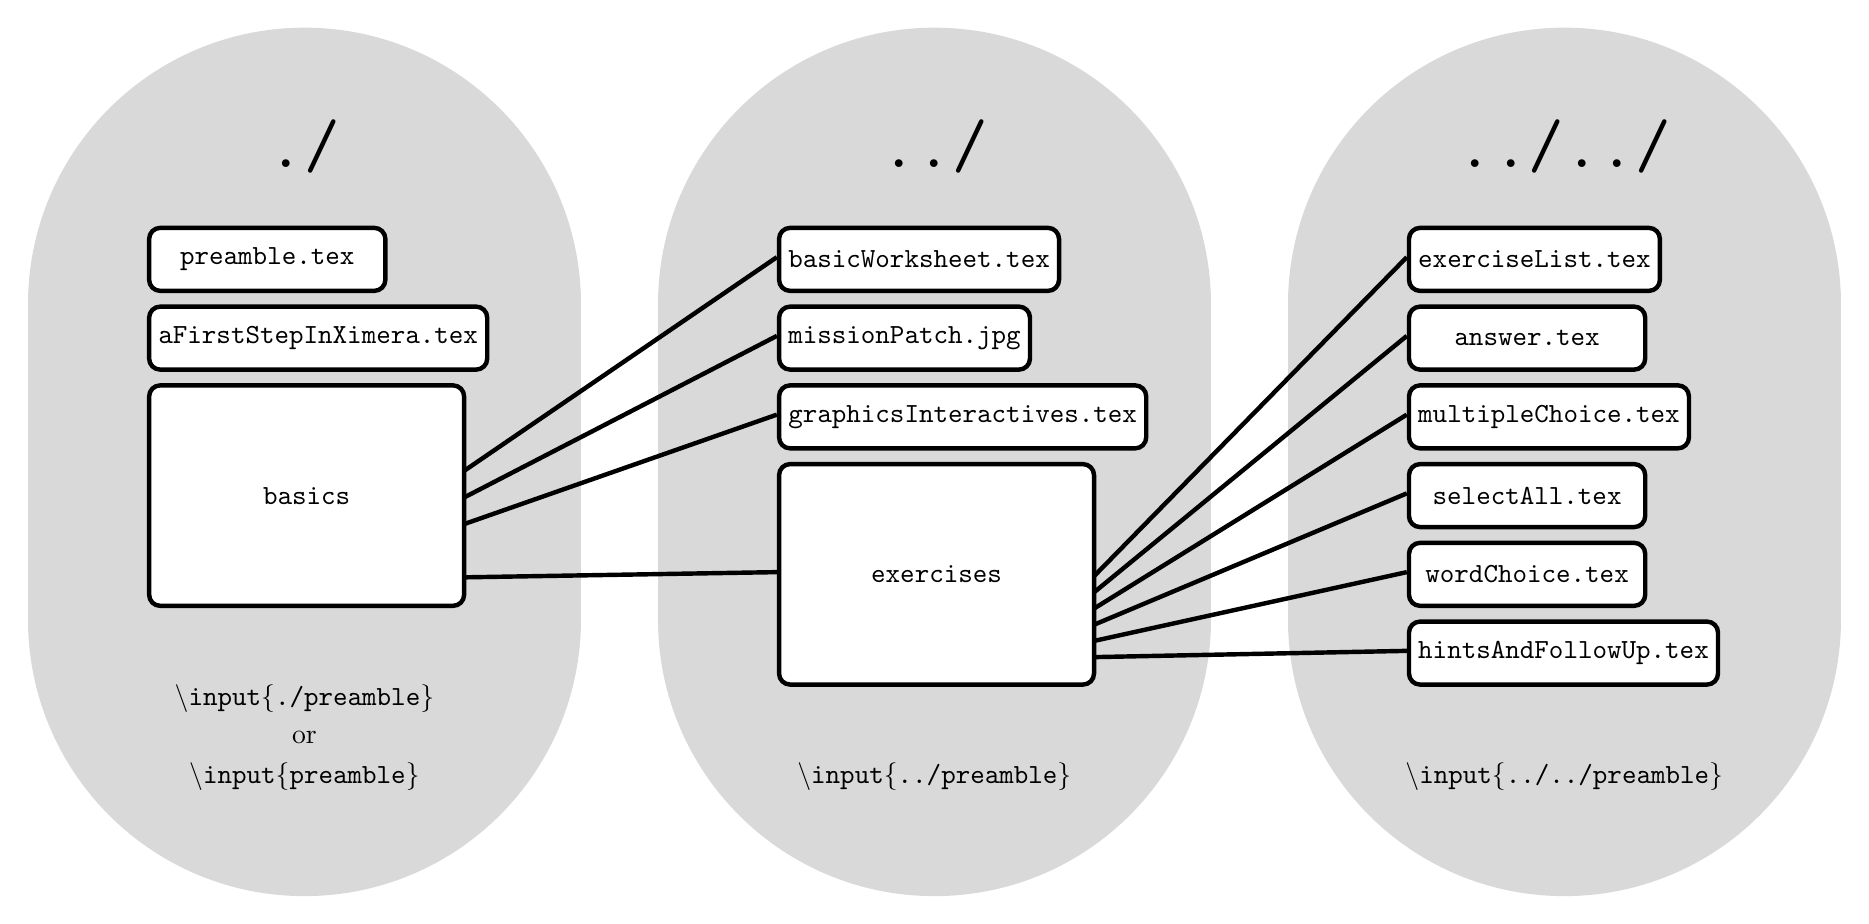
\begin{tikzpicture}
      % Define styles for nodes
      \tikzstyle{document} = [anchor=north west,draw, rounded corners,
      rectangle,
      minimum width=3cm,fill=white, minimum height=.8cm, ultra
      thick,font=\ttfamily]
      \tikzstyle{folder} = [anchor=north west,draw, rectangle, rounded corners,
      minimum width=4cm,fill=white, minimum height=2.8cm, ultra
      thick,font=\ttfamily]

      % Thick grey lines
      \draw[line width=200pt,white!85!black,line cap=round] (2,2) -- (2,-2);
      \draw[line width=200pt,white!85!black,line cap=round] (10,2) -- (10,-2);
      \draw[line width=200pt,white!85!black,line cap=round] (18,2) -- (18,-2);

      % Connections
      \draw[ultra thick] (2,-1.5) -- (8,2.6);
      \draw[ultra thick] (2,-1.5) -- (8,1.6);
      \draw[ultra thick] (2,-1.5) -- (8,.6);
      \draw[ultra thick] (2,-1.5) -- (8,-1.4);

      \draw[ultra thick] (11,-2.5) -- (16,2.6);
      \draw[ultra thick] (11,-2.5) -- (16,1.6);
      \draw[ultra thick] (11,-2.5) -- (16,.6);
      \draw[ultra thick] (11,-2.5) -- (16,-.4);
      \draw[ultra thick] (11,-2.5) -- (16,-1.4);
      \draw[ultra thick] (11,-2.5) -- (16,-2.4);

      % Symbols at top
      \node at (2,4) {\Huge \tt ./};
      \node at (10,4) {\Huge \tt ../};
      \node at (18,4) {\Huge \tt ../../};

      % Define the folders at top level
      \node[document] at (0,3) {preamble.tex};
      \node[document] at (0,2) {aFirstStepInXimera.tex};
      \node[folder] at (0,1) {basics};

      % Define the documents in the basics folder
      \node[document] at (8,3) {basicWorksheet.tex};
      \node[document] at (8,2) {missionPatch.jpg};
      \node[document] at (8,1) {graphicsInteractives.tex};
      \node[folder] at (8,0) {exercises};

      % Define the documents in the exercises folder
      \node[document] at (16,3) {exerciseList.tex};
      \node[document] at (16,2) {answer.tex};
      \node[document] at (16,1) {multipleChoice.tex};
      \node[document] at (16,0) {selectAll.tex};
      \node[document] at (16,-1) {wordChoice.tex};
      \node[document] at (16,-2) {hintsAndFollowUp.tex};

      % paths at bottom
      \node at (2,-3) {\tt\textbackslash input\{./preamble\}};
      \node at (2,-3.5) {or};
      \node at (2,-4) {\tt\textbackslash input\{preamble\}};
      \node at (10,-4) {\tt\textbackslash input\{../preamble\}};
      \node at (18,-4) {\tt\textbackslash input\{../../preamble\}};
    \end{tikzpicture}
  }
\end{center}
\pdfOnly{\twocolumn}

\begin{verbatim}
%% where to find images
\graphicspath{
{./}
{./graphicsVideosAndInteractives/}
}
\end{verbatim}

\end{document}